\documentclass{beamer}
\usepackage{graphicx}
\usepackage{amsmath}
\usepackage{bm}
\graphicspath{{Images/}}
\mode<presentation>
\title{Introduction to Finite Element and CFD}
\institute{Corvid Technologies}
\date{2017-05-16}

\begin{document}
\frame{\titlepage}

\section{Introduction}
\begin{frame}{Introduction}
\begin{block}{Disclaimer}
	This is meant to be a brief overview of Computational Structural and Fluid Dynamics.
	All of this Material is taken from:
	\begin{enumerate}
		\item \underline{Nonlinear Finite Elements for Continua and Structures} by Ted Belytschko 
		\item \underline{Computational Gas Dynamics} by Culbert Laney
	\end{enumerate}
\end{block}
\begin{block}{Topics To Be Covered}
\begin{itemize}
	\item Lagrangian and Eularian Frames
	\item Continuum Mechanics Overview
	\item Conservation Equations
	\item Weak Forms and Shape Functions
	\item Computational Fluid Dynamics Overview
\end{itemize}
\end{block}
\end{frame}

\section{Lagrangian and Eularian Frames}
\begin{frame}{Lagrangian and Eularian Frames}
\begin{block}{Notation}
	Because there are two different frames of reference, we will need
	two vectors to represent the position 
	\begin{itemize}
		\item $\vec{X}$ for the Lagrangian Position
		\item $\vec{x}$ for the Eularian Position
	\end{itemize}		
\end{block}
\begin{figure}[!ht]
	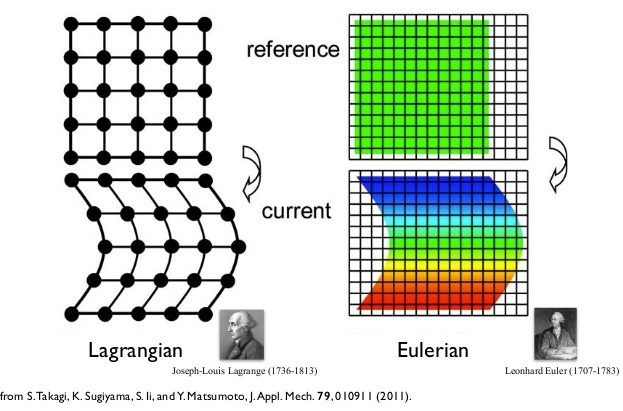
\includegraphics[scale=0.5]{LE2}
	\caption{Blatantly stolen from the internet}
	\label{fig:LE}
\end{figure}
\end{frame}
\section{Overview of Continuum Mechanics}
\begin{frame}{Overview of Continuum Mechanics}
	Let the relationship between the Lagrangian and Eularian coordinates be:
	\begin{subequations}
		\begin{equation}\label{eq:phi}		
			\vec{x}=\boldsymbol{ \phi}(\vec{X})
		\end{equation}
		\begin{equation}
			d\vec{x}=\frac{\partial \boldsymbol{\phi}}{\partial\vec{X}}d\vec{X}
		\end{equation}
		\begin{equation}
			F_{ij}=\frac{\partial \phi_{i}}{\partial X_{j}}
		\end{equation}
	\end{subequations}
\begin{block}{Deformation Gradient}
$\mathbf{F}$ is known as the \textbf{Deformation Gradient Tensor} and it is probably the most important quantitiy in continuum mechanics. It relates a material (Lagrangian) infinitesimal vector $\mathbf{dX}$ to the spatial (Eularian) vector $\mathbf{dx}$. It is very often used in development of constitutive equations and as well as measures of strain. For instance the Green-Lagrange Strain Tensor is given by:
\end{block}
\begin{equation}
	\mathbf{E}=\frac{1}{2}(\mathbf{F}^{T}\mathbf{F}-\mathbf{I})
\end{equation}
\end{frame}
\begin{frame}{Overview of Continuum Mechanics}
	\begin{figure}
		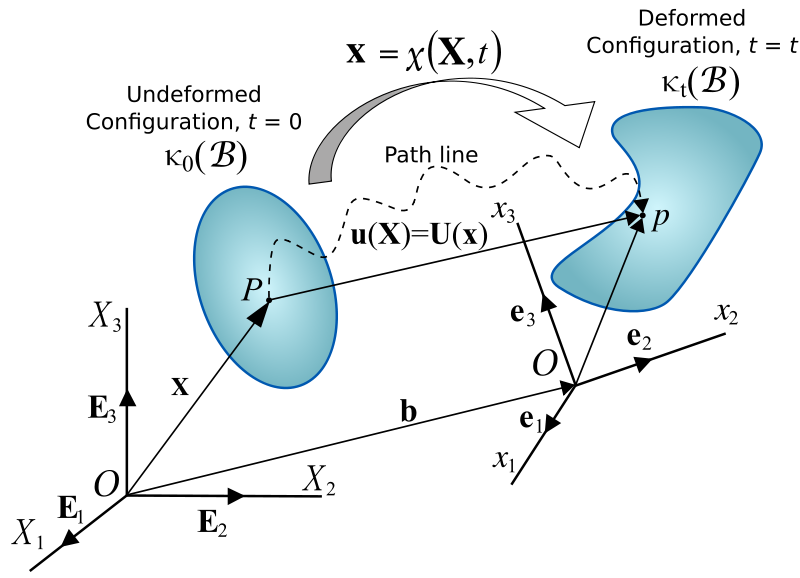
\includegraphics[scale=0.25]{Deform}
		\caption{Deformation (Remember when your teacher told you not to use Wikipedia?)}
	\end{figure}
	
\end{frame}
\subsection{Conservation Equations}
\begin{frame}{Conservation Equations}
	The three physical quantities that we are trying to conserve:
	\begin{enumerate}
		\item mass
		\item linear momentum
		\item energy
	\end{enumerate}
\vskip 1cm
	Each of these conservation equations can be represented withing the Lagrangian or the Eularian Frame 	work. Keeping in mind that we can always jump between them and they represent the same physical process.
\end{frame}

\subsubsection{Conservation of Mass}
\begin{frame}{Conservation of Mass}
The detailed derivation of this can be found in Belytschko, \textbf{Section 3.5.4}
	\begin{block}{Lagrangian}
		Lagrangian conservation of mass is given by:
		\begin{subequations}
			\begin{equation}
				\rho(\mathbf{X},t)J(\mathbf{X},t)=\rho_{0}(\mathbf{X})
			\end{equation}
			\begin{equation}
				J(\mathbf{X},t)=det|\mathbf{F}(\mathbf{X},t)|
			\end{equation}
		\end{subequations}
	\end{block}
\begin{block}{Eularian}
	Eularian conservation of mass is given by:
	\begin{equation}
		\frac{\partial \rho(\mathbf{x},t)}{\partial t}+\nabla\cdot[\rho(\mathbf{x},t)\mathbf{v}						(\mathbf{x},t)]
	\end{equation}
\end{block}
\end{frame}

\subsubsection{Conservation of Momentum}

\begin{frame}{Conservation of Momentum}
This is of course nothing but $\mathbf{F}=m\mathbf{a}$.
\linebreak
We will need to utilize the concept of body force $\mathbf{b}(\mathbf{X/x},t)$
and the Cauchy Tensor $\mathbf{\sigma}(\mathbf{x},t)$. Notice that $\mathbf{\sigma}$ is only defined in the spatial (Eularian) frame. Stresses require careful treatment with respect to the reference frame. Although this is out of scope of this presentation, the 2nd Piola Kirchhoff $\mathbf{S}(\mathbf{X},t)$ is the stress in the material (Lagrangian) configuration.
\end{frame}

\begin{frame}{Conservation of Momentum}
\begin{block}{Lagrangian}
	\begin{equation}
		\rho(\mathbf{X},t)\frac{\partial\mathbf{v}(\mathbf{X},t)}{\partial t}=\nabla\cdot\bm{\sigma}(\mathbf{x},t)+\rho(\mathbf{X},t)\mathbf{b}(\mathbf{X},t)
	\end{equation}
	Note that $\sigma$ is in the spatial and not the material coordinates
\end{block}

\begin{block}{Eularian}
	\begin{equation}
		\frac{D(\rho\mathbf{v})}{Dt}=div(\bm{\sigma)}+\rho\mathbf{b}
	\end{equation}
	For simplicity, the spatial coordinates were omited, but all are functions of $\mathbf{x}$
\end{block}
\end{frame}

\subsubsection{Conservation of Energy}

\begin{frame}{Conservation of Energy}
These are getting really complicated, so conservation of energy is only shown in the Eularian Frame work.
This is derived in more detail in Belytschko \textbf{Section 3.5.9}
	\begin{equation}
		\rho\frac{ Dw^{int} }{Dt}=\mathbf{D}:\bm{\sigma}-\nabla\cdot\mathbf{q}+\rho s
	\end{equation}
	Note the use of the velocity gradient $\mathbf{D}$. The definition of $\mathbf{D}$ comes from the rate of deformation tensor $\mathbf{L}$
	\begin{subequations}
		\begin{equation}
			\mathbf{L}=\dot{\mathbf{F}}\cdot\mathbf{F}^{-1}
		\end{equation}
		\begin{equation}
			\dot{\mathbf{F}}=\frac{\partial \mathbf{v}}{\partial \mathbf{X}}
		\end{equation}
		\begin{equation}
			\mathbf{L}=\frac{1}{2}[\mathbf{L}+\mathbf{L}^{T}]+\frac{1}{2}[\bm{L}-\bm{L}^{T}];\
			\bm{L}=\bm{D}+\bm{W}
		\end{equation}
	\end{subequations}
\end{frame}

\section{Developing the Weak Form}
\begin{frame}{Developing the Weak Form}

\end{frame}
\end{document}